%
% This is a borrowed LaTeX template file for lecture notes for CS267,
% Applications of Parallel Computing, UCBerkeley EECS Department.
% Now being used for CMU's 10725 Fall 2012 Optimization course
% taught by Geoff Gordon and Ryan Tibshirani.  When preparing 
% LaTeX notes for this class, please use this template.
%
% To familiarize yourself with this template, the body contains
% some examples of its use.  Look them over.  Then you can
% run LaTeX on this file.  After you have LaTeXed this file then
% you can look over the result either by printing it out with
% dvips or using xdvi. "pdflatex template.tex" should also work.
%

\documentclass[twoside]{article}
\setlength{\oddsidemargin}{0.25 in}
\setlength{\evensidemargin}{-0.25 in}
\setlength{\topmargin}{-0.6 in}
\setlength{\textwidth}{6.5 in}
\setlength{\textheight}{8.5 in}
\setlength{\headsep}{0.75 in}
\setlength{\parindent}{0 in}
\setlength{\parskip}{0.1 in}

%
% ADD PACKAGES here:
%

\usepackage{amsmath,amsfonts,graphicx}

%
% The following commands set up the lecnum (lecture number)
% counter and make various numbering schemes work relative
% to the lecture number.
%
\newcounter{lecnum}
\renewcommand{\thepage}{\thelecnum-\arabic{page}}
\renewcommand{\thesection}{\thelecnum.\arabic{section}}
\renewcommand{\theequation}{\thelecnum.\arabic{equation}}
\renewcommand{\thefigure}{\thelecnum.\arabic{figure}}
\renewcommand{\thetable}{\thelecnum.\arabic{table}}

%
% The following macro is used to generate the header.
%
\newcommand{\lecture}[4]{
   \pagestyle{myheadings}
   \thispagestyle{plain}
   \newpage
   \setcounter{lecnum}{#1}
   \setcounter{page}{1}
   \noindent
   \begin{center}
   \framebox{
      \vbox{\vspace{2mm}
    \hbox to 6.28in { {\bf EE302 - Feedback Systems
	\hfill Spring 2019} }
       \vspace{4mm}
       \hbox to 6.28in { {\Large \hfill Lecture #1 \hfill} }
       \vspace{2mm}
       \hbox to 6.28in { {\it Lecturer: #2 \hfill } }
      \vspace{2mm}}
   }
   \end{center}
   \markboth{Lecture #1}{Lecture #1}

   \vspace*{4mm}
}
%
% Convention for citations is authors' initials followed by the year.
% For example, to cite a paper by Leighton and Maggs you would type
% \cite{LM89}, and to cite a paper by Strassen you would type \cite{S69}.
% (To avoid bibliography problems, for now we redefine the \cite command.)
% Also commands that create a suitable format for the reference list.
\renewcommand{\cite}[1]{[#1]}
\def\beginrefs{\begin{list}%
        {[\arabic{equation}]}{\usecounter{equation}
         \setlength{\leftmargin}{2.0truecm}\setlength{\labelsep}{0.4truecm}%
         \setlength{\labelwidth}{1.6truecm}}}
\def\endrefs{\end{list}}
\def\bibentry#1{\item[\hbox{[#1]}]}

%Use this command for a figure; it puts a figure in wherever you want it.
%usage: \fig{NUMBER}{SPACE-IN-INCHES}{CAPTION}
\newcommand{\fig}[3]{
			\vspace{#2}
			\begin{center}
			Figure \thelecnum.#1:~#3
			\end{center}
	}
% Use these for theorems, lemmas, proofs, etc.
\newtheorem{theorem}{Theorem}[lecnum]
\newtheorem{lemma}[theorem]{Lemma}
\newtheorem{proposition}[theorem]{Proposition}
\newtheorem{claim}[theorem]{Claim}
\newtheorem{corollary}[theorem]{Corollary}
\newtheorem{definition}[theorem]{Definition}
\newenvironment{proof}{{\bf Proof:}}{\hfill\rule{2mm}{2mm}}

% **** IF YOU WANT TO DEFINE ADDITIONAL MACROS FOR YOURSELF, PUT THEM HERE:

\begin{document}

% Lecture Details
\lecture{13}{Asst. Prof. M. Mert Ankarali}

\par 

\section{PID Control Analysis \& Design with Root-Locus}

Let's assume that we would like you to design a 
controller for the following second order plant
transfer function
%
\begin{align*}
  G(s) = \frac{1}{(s+1) (s+3)}
\end{align*}
%
The requirements of the closed-loop system are
%
\begin{itemize}
  \item Minimum possible settling time ($\%2$)
  \item Minimum steady-state error 
  \item Minimum possible over-shoot
\end{itemize}

\subsection{Proportional (P) Controller}

Let's first design a P controller, $C(s) = K$. Let's start with steady-state error
performance. Plant is a type-one system and controller is a static
gain thus unit step and unit ramp steady-state error can be computed as
%
\begin{align*}
   \mathrm{Step:}& \quad e_{ss} = \frac{1}{1 + K_P/3}
\\
\mathrm{Step:}& \quad e_{ss} = \infty
\end{align*} 
%
We can see that unit-ramp error is $\infty$ regardless of $K_P$,
where as we can reduce the steady-state error by increasing 
proportional gain $K_P$. Now let's draw root locus and
comment on settling time and over-shoot performance. 

\vspace{12 pt}

  \begin{minipage}[h]{1\linewidth}
    \begin{center}
      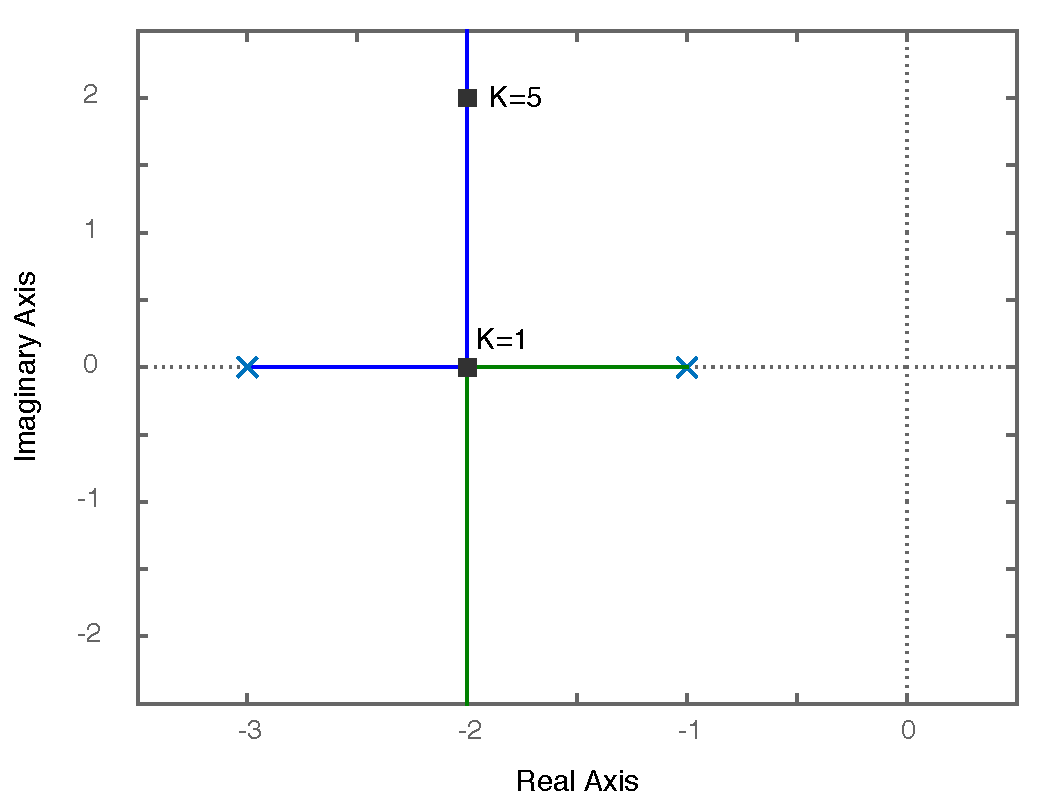
\includegraphics[width=0.5\textwidth]{Plocus}
    \end{center}
  \end{minipage}

\vspace{12 pt}

Based on root-locus plot we can see that best convergence rate 
achieved with $\sigma = -2$, for which the approximate settling time
is $2 s.$ When $K = 1$, system becomes critically damped. When we
further increase the gain, real part of the poles do not change,
however oscillations starts and grows with $K_P$. Obviously, we
should choose a gain $K_P > 1$, however after that point
theres is a trade-off between over-shoot and settling time
performance. Let's choose two candidate locations, $p_{1,2}^{(1)} = -2$
and $p_{1,2}^{(1)} = -2 \pm 2 j$. Table below details
the gain values at these pole locations, unit-step steady-state errors,
and estimated settling time and maximum over-shoot values. 

\vspace{6pt}
\begin{minipage}[h]{1\linewidth}
\begin{center}
\begin{tabular}{|c | c | c | c | c  |}
\hline
$p_{1,2}$ & $K_P$ & $e_{ss}$ & $t_s$ & $M_P$
\\ \hline
-2 & 1 & 0.75 & 2 & 0
\\ \hline
$-2 \pm 2 $  & 5 & 0.375 & 2 & 0.04
\\ \hline
\end{tabular}
\end{center}
\end{minipage}
\vspace{6pt}

We verify that both steady-state and transient performance increases
with larger $K_P$. However, we can also see that settling time
estimation for $K_P = 5$ has a larger error, which expected
since the poles are close to each other thus violates the
dominant pole assumption. If we consider the values in the table, 
it seems to be reasonable to choose $K_P = 5$ since it provides a
much better steady-state performance, of course if existing
of an small overs-shoot is not a major problem for the design.
Now let's plot step-responses of the closed loop system for
both cases. 

\vspace{12 pt}

  \begin{minipage}[h]{1\linewidth}
    \begin{center}
      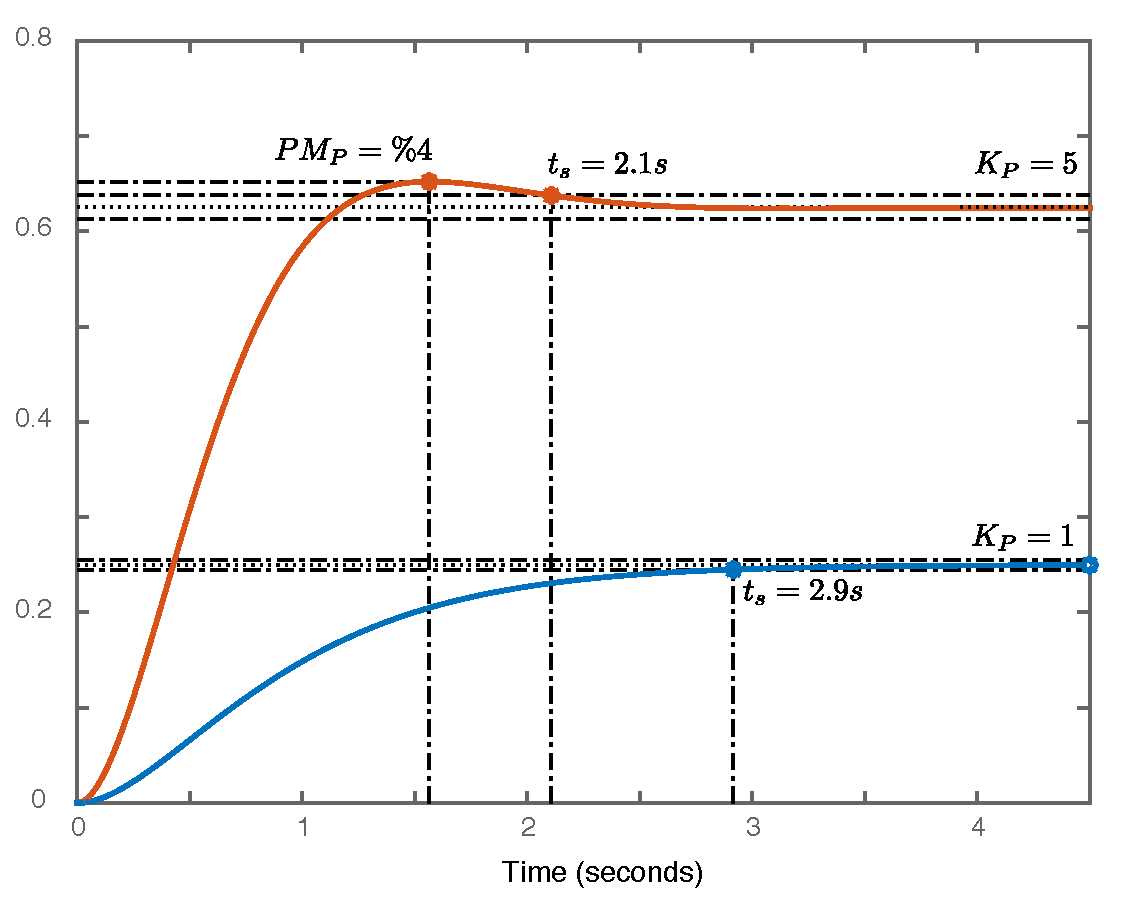
\includegraphics[width=0.5\textwidth]{Pcont}
    \end{center}
  \end{minipage}

\vspace{12 pt}

We verify most of our theoretical findings with the only
exception about the settling time for $K_P = 1$, which is
larger then the estimation. In conclusion, $K_P = 5$ is a 
good choice for overall requirements. 

\subsection{Proportional Derivative (PD) Controller}

Now let's design a PD controller. First make some change of
variables and re-write the PD controller in a different form.
%
\begin{align*}
 C(s) = K_P + K_D s = K_D \left( s + \frac{K_P}{K_D} \right) = K_D (s
  + \alpha)
\end{align*}
%
We can see that PD controller introduces an extra zero to the
open loop transfer function. Let's compute the steady-state error performance. 
%
\begin{itemize}
\item Unit step: $e_{ss} = \frac{1}{1 + K_P/ 3} = \frac{1}{1 + \alpha K_D/ 3}$, 
\item Unit ramp: $e_{ss} = \infty$
\end{itemize}
 %
Technically in classical PD form $K_D$ has no effect on steady-state
performance. However if we adopt the second form with $\alpha$
and fix $\alpha$ first, then as we increase $K_D$ steady-state error
will decrease. Now let's fix $\alpha = 4 = \frac{K_P}{K_D}$, and draw 
the root-locus. 

\vspace{12 pt}

  \begin{minipage}[h]{1\linewidth}
    \begin{center}
      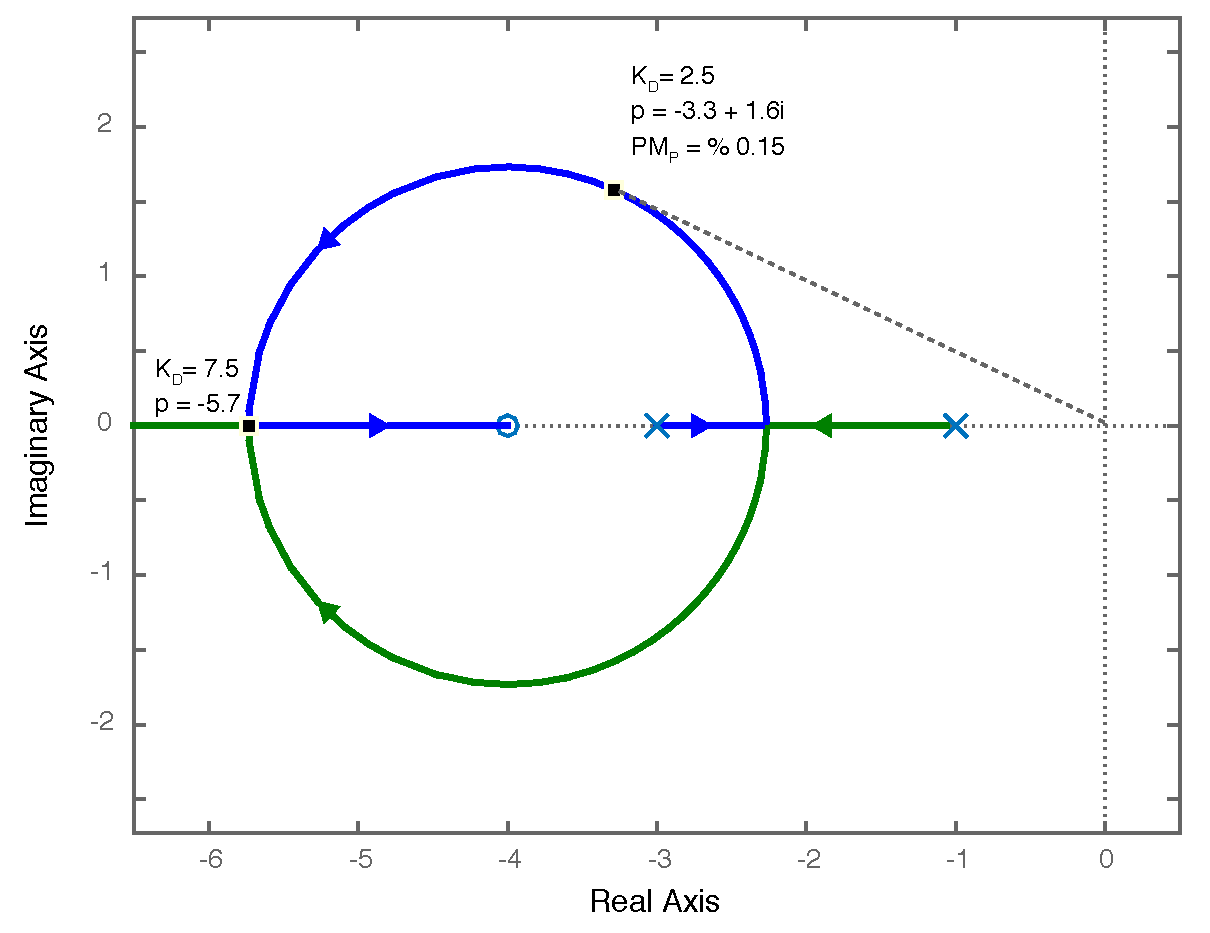
\includegraphics[width=0.4\textwidth]{PDlocus}
    \end{center}
  \end{minipage}

\vspace{12 pt}

We think that the improvement of added zero is very clear.
If we carefully look at the root-locus, we can see that
at the pole location that gives the worst maximum over-shoot
performance, maximum percent over-shoot is only $\% 0.15$,
moreover overs-shoot completely disappears when $K_D \geq 7.5$.
The best settling/convergence time performance occurs at the
break-in point which has an approximate gain of $K_D = 7.5$,

Table below details the P and D gain values at this pole locations, 
closed-pole locations,  unit-step steady-state error, and estimated
settling time value. 

\vspace{6pt}
\begin{minipage}[h]{1\linewidth}
\begin{center}
\begin{tabular}{|c | c | c | c | c  |}
\hline
$K_P$ &$K_D$ & p & $e_{ss}$ & $t_s [s]$ 
\\ \hline
30 & 7.5& -5.7 & 0.09 & 0.7
\\ \hline
\end{tabular}
\end{center}
\end{minipage}
\vspace{6pt}

Now let's compare this PD controller (with $(K_P,K_D) = (30,7.5)$)
and the previously designed P controller (with $(K_P,K_D) = (5,0)$)
by simulating the step responses. 

\vspace{12 pt}

  \begin{minipage}[h]{1\linewidth}
    \begin{center}
      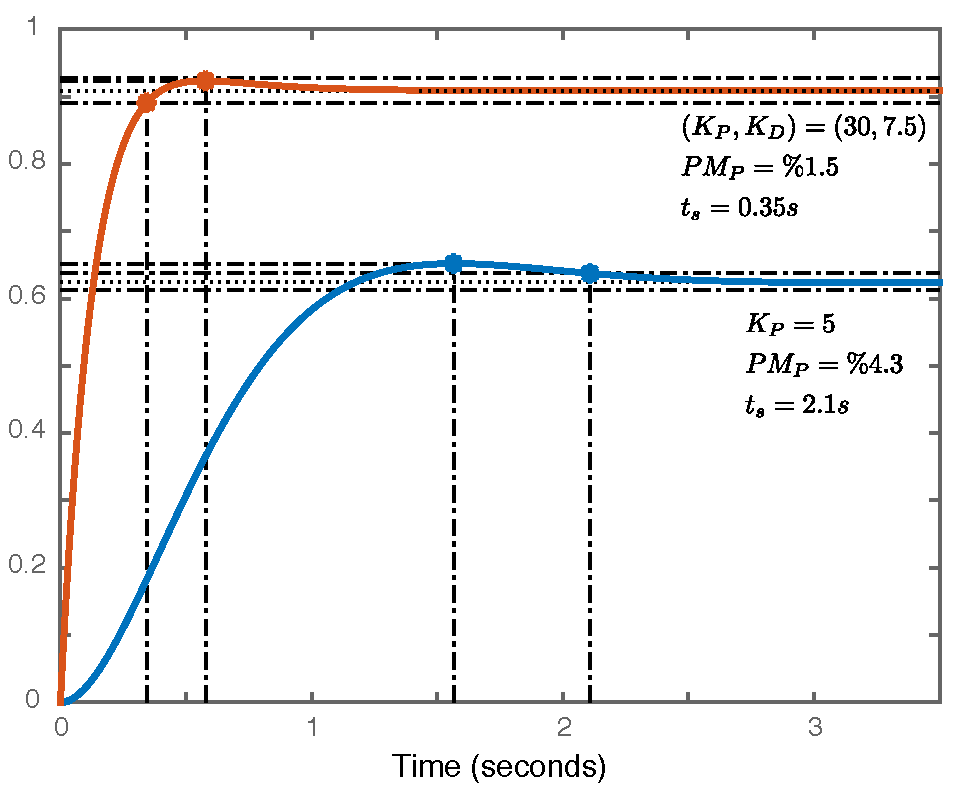
\includegraphics[width=0.4\textwidth]{PDvsP}
    \end{center}
  \end{minipage}

\vspace{12 pt}

We can see that PD control policy outperforms 
the P controller in every category. 

On the other hand, interestingly we expected no over-shoot with
thet PD controller, yet we still observe some over-shoot 
at the output. In addition to this, actual settling 
time is approximatelly half of our previous estimation. 
The discrepancies between the transient characteristics between
simulation and estimated values occurs due the
effectx of extra zero in the closed-loop transfer function. 

\subsection{Integral (I) Controller}

Now let's analyze how a pure integral controller affects 
the proposed system using root-locus analysis. 

%
\begin{align*}
 C(s) = \frac{K_I}{s} \quad &, \quad G(s) = \frac{1}{(s+1) (s+3)}
\\
G_{OL}(s) = \frac{1}{s (s+1) (s+3)} \quad &, \quad K = K_I
\end{align*}
%
We already know that steady-state performance is affected
positively with an Integral controller
%
\begin{itemize}
\item Unit step: $e_{ss} = 0$
\item Unit ramp: $e_{ss} = \frac{3}{K_I}$
\end{itemize}
 %
Now let's analyze the affects on transient performance
and stability using root-locus diagram
%
\vspace{12pt}

\begin{minipage}[h]{0.5\linewidth}
    \begin{center}
      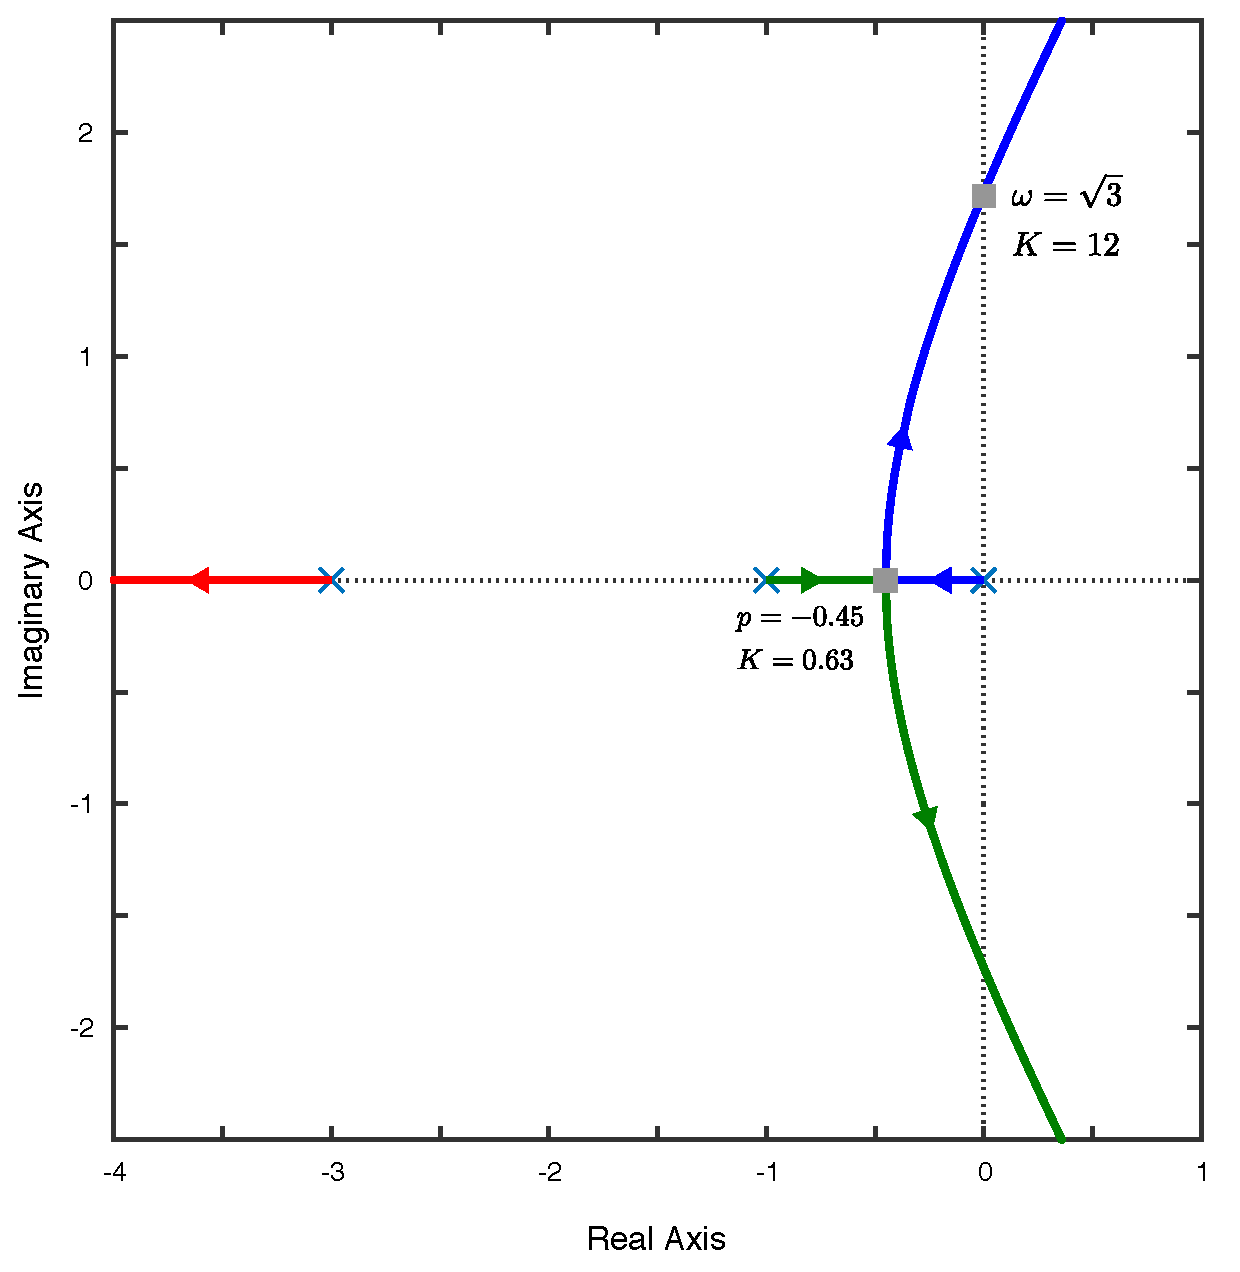
\includegraphics[width=0.95\textwidth]{Ilocus}
    \end{center}
\end{minipage}
\begin{minipage}[h]{0.5\linewidth}
	Break-away point
	\begin{align*}
	& 3 \sigma_{b}^2 + 8 \sigma_b + 3 = 0 
	\\
	& \sigma_{b,1} = - 0.45  \ \rightarrow \ \mathrm{OK} \quad ,
          \quad K = 0.63
	\\
	& \sigma_{b,2} =  -2.2 \ \rightarrow \ \mathrm{NO}
	\end{align*}
	Imaginary axis crossing
	\begin{align*}
	& D(j \omega) + K_I N(j \omega) = 0 \\ 	 
	& (j \omega)^3 + 4 (j \omega)^2 + 3 (j \omega) + K_I = 0 \\ 
	& (K - 4 \omega^2) + (3 \omega - \omega^3) j = 0
	\\ & \Rightarrow \omega = \sqrt{3}  \quad , \ K = 12
	\end{align*}
\end{minipage}

\vspace{12pt}

We can make the following observations
%
\begin{itemize}
 \item Closed-loop system becomes unstable for $K_I > 6$. Note that
   with a P controller closed loop system was always stable for $K_P >0$
  \item Best settling time that can be achieved with an I controller
    is approximately, $t_{s} = 9 s$, which is quite bad compared to
   the simple P-controller. 
\end{itemize}
% 
In conclusion, integral action improves steady-state performance, but
it degrades the stability and transient performance. 

\subsection{Proportional Integral (PI) Controller}

Now let's design a PI controller. First make some change of
variables and re-write the PI controller in a different form.
%
\begin{align*}
 C(s) = K_P + K_I \frac{1}{s} = K_P \left( \frac{ s + K_I / K_P }{s}
  \right) = K_P \left( \frac{ s + \alpha }{s} \right)
\end{align*}
%
We can see that PI controller introduces an extra zero to the
open loop transfer function and a pole at the origin. 
We know that the steady-state error performance characteristics. 
of a PI controller is same with an I controller. 

Now let's fix $\alpha = 2 = \frac{K_I}{K_P}$, and draw 
the root-locus w.r.t $K_P$. Note that 
%
\begin{align*}
  G_{OL}(s) = \frac{s+2}{s (s+1) (s+3)}
\end{align*}


\begin{minipage}[h]{0.5\linewidth}
    \begin{center}
      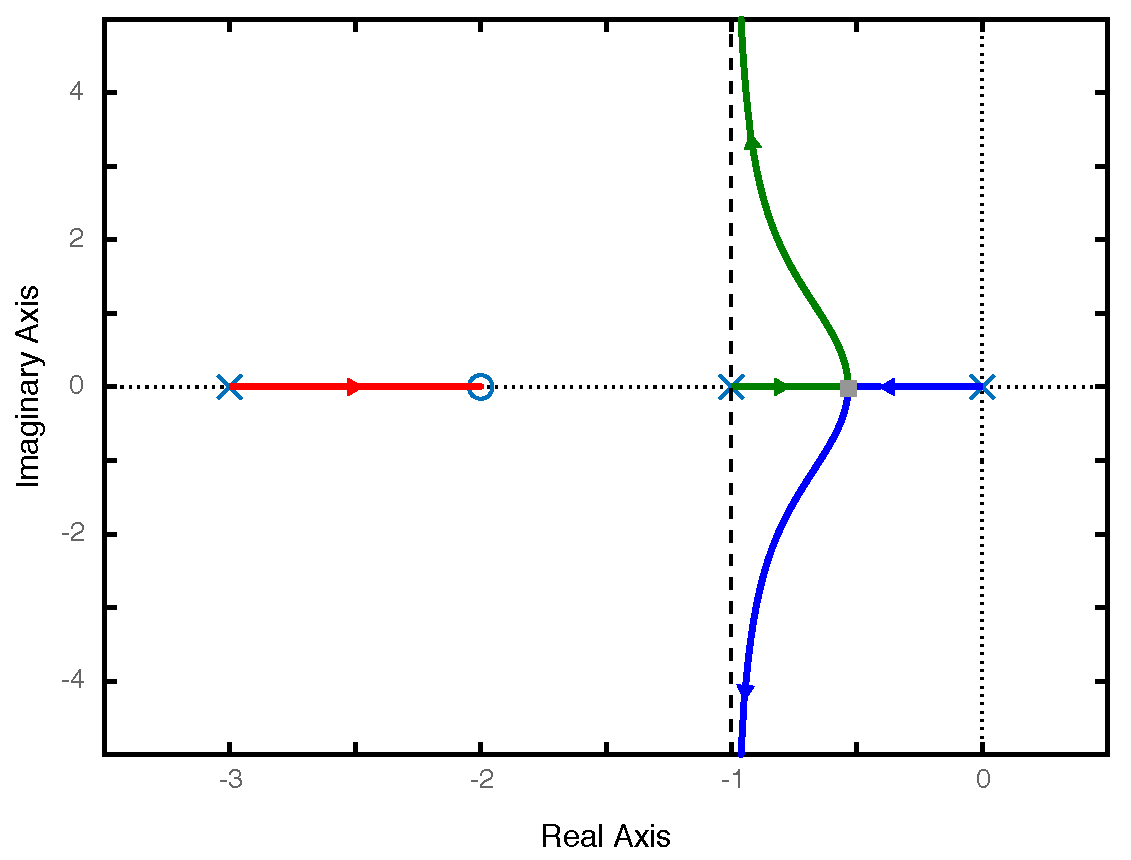
\includegraphics[width=0.95\textwidth]{PIlocus}
    \end{center}
\end{minipage}
\begin{minipage}[h]{0.5\linewidth}
	Break-away point
	\begin{align*}
	& 2 \sigma_{b}^3 + 10 \sigma_{b}^2 + 16 \sigma_b + 6 = 0 
	\\
	& \sigma_{b,1} = - 0.53  \ \rightarrow \ \mathrm{OK} \quad ,
          \quad K = 0.42
	\\
	& \sigma_{b,2} =  -2.2 \pm 0.8 j \ \rightarrow \ \mathrm{NO}
	\end{align*}
\end{minipage}

We can make the following observations
%
\begin{itemize}
 \item Closed-loop system is stable for $K_P > 0$ for this choice of
   $\alpha$. 
  \item Best settling time that can be achieved with this PI controller
    is approximately, $t_{s} = 4 s$, but this is achieved when $K \to
    \infty$.
  \item Best settling time value with this PI controller is the
    approximately double of the best settling time value of the
    P controller.
  \item System is approximately acts like a second-order over-damped
   system when $K_P \in (0,0.42)$, where as acts like a a second-order 
   under-damped system when $K_P \in (0.42,\infty)$. 
   \item Oscillations and over-shoot increases as we increase $K_P$. 
   This there is a trade-off between settling time and over-shoot
   performance. 
\end{itemize}
% 
In conclusion, PI controller has superior steady-state performance
compared to P and PD controllers, however there exist substantial 
transent performance drop even compared to simple P controller. 

Now let's choose $K_P = 2$, then we can find that $K_I = 4$.
Now let's compre this PI controller $(K_P , K_I) = (2,4)$ with our
previously chosen P controller $(K_P , K_I) = (5,0)$ by simulating
the step-responses. 

\vspace{12 pt}

  \begin{minipage}[h]{1\linewidth}
    \begin{center}
      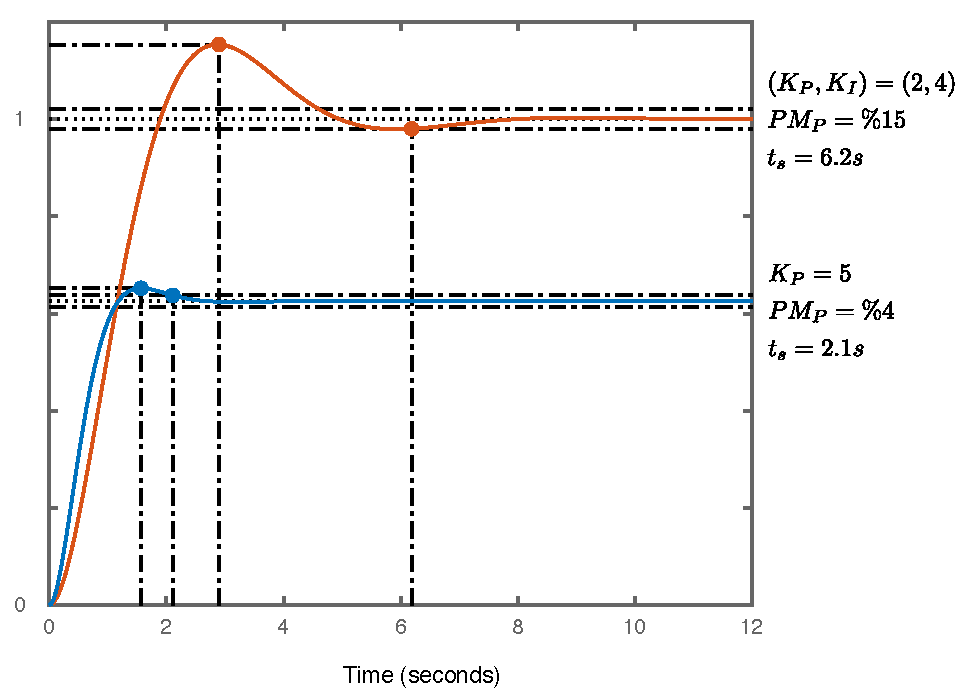
\includegraphics[width=0.5\textwidth]{PvsPI}
    \end{center}
  \end{minipage}

\vspace{12 pt}

It is obvious that while PI controller has a superior steady-state
performance, P controller provides much better transient
characteristics. 

\textbf{Practice Question:} Choose $\alpha$ from this set  $\lbrace 4,
\ -1.2, \  0.8  \rbrace$, and draw the root-locus diagrams for each
$\alpha$. Comment on the results in terms of overall transient performance
based on the root locus diagrams.

\subsection{Proportional Integral Derivative (PID) Controller}

If one is not satisfied with the transient characteristics of a
P-controller but also would like to eliminiate steady-state error
fot the unit step input, he/she can design a PID controller. 

First make some change of variables and re-write the PID controller in a different form.
%
\begin{align*}
 C(s) &= K_D s + K_P + K_I \frac{1}{s} = K_D  \left( s +   (K_P/K_D) +
  (K_I/K_D) \frac{1}{s} \right)\\
&= K_D  \left( s^2 +   (K_P/K_D) s  + (K_I/K_D) \right) \frac{1}{s}
\end{align*}
%
We can see that a PID controller has a second order numerator
dynamics, and it is possible to have two real zeros, or two complex
conjugate zeros. In general, PID gains are chosen such that 
numerator has two zeros
\begin{align*}
 C(s) &= K_D \frac{(s+\alpha) (s + \beta)}{s}
\end{align*}
%
We know that PID controller has same stead-state performance
characteristics with PI and I controllers. Now let's choose $\alpha =
2$ and $\beta = 4$ and draw the root locus w.r.t. $K_D$.

\vspace{12 pt}

  \begin{minipage}[h]{1\linewidth}
    \begin{center}
      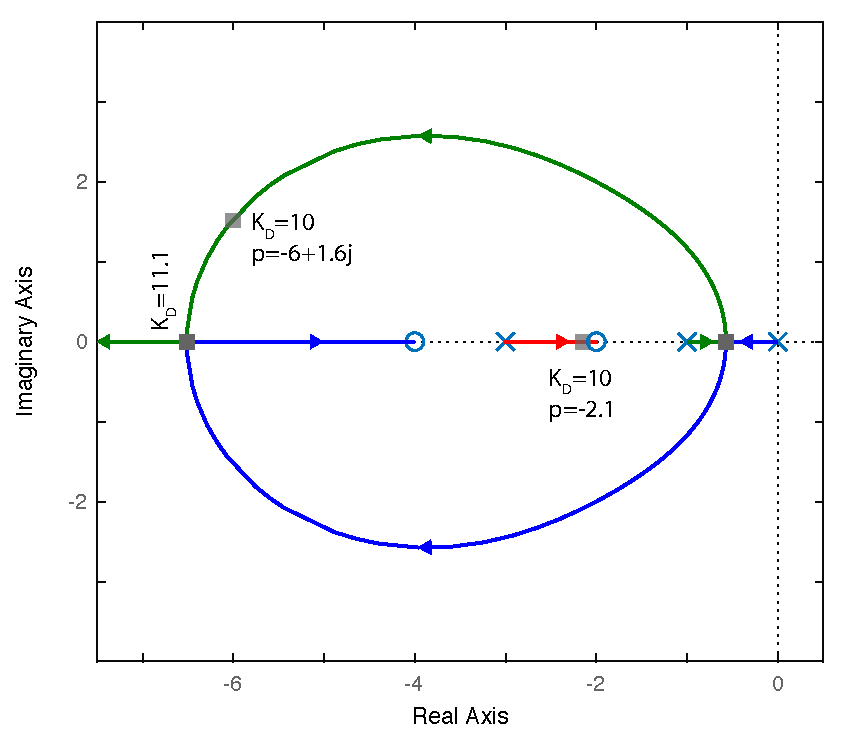
\includegraphics[width=0.45\textwidth]{PIDlocus}
    \end{center}
  \end{minipage}

\vspace{12 pt}

Unlike the root-locus plots of previous cases, it is harder to
have an idea about what is good for transient performance.
It seems that as $K_D \nearrow$, one pole on the real axis 
move towards imaginary axis and stops at $\sigma = -2$ when
$K \to \infty$, where as other two poles deviates from the imaginary
axis when $K_D \nearrow$. Let's choose $K_D = 10$ which marked 
on the root-locus plot. In this case poles of the closed-loop system 
takes the form $p_1 = -2.1$ and $p_{2,3} = -6 \pm 1.6 j$. We 
may conclude that the system is approximatelly first order since
the single pole is much closer to the real-axis. In this case, we
expect settling time as $t \approx 1.9 s$. Note that this settling time
value is slightly better then the best settling time value that is
satisfied with a P-controller. Moreover we expect that over-shoot would
be negligible (less than $\% 0.001$).

When $K_D = 10$, we have 

\begin{align*}
&s^2 +   (K_P/K_D) s  + (K_I/K_D) = (s+2)(s+4) = s^2 + 6 s + 8
\\
&K_P = 60
\\
&K_I = 80
\end{align*}

Now let's simulate this PID controller and previously designed PD
controller and compre the transient and steady state performances.

\vspace{12 pt}

  \begin{minipage}[h]{1\linewidth}
    \begin{center}
      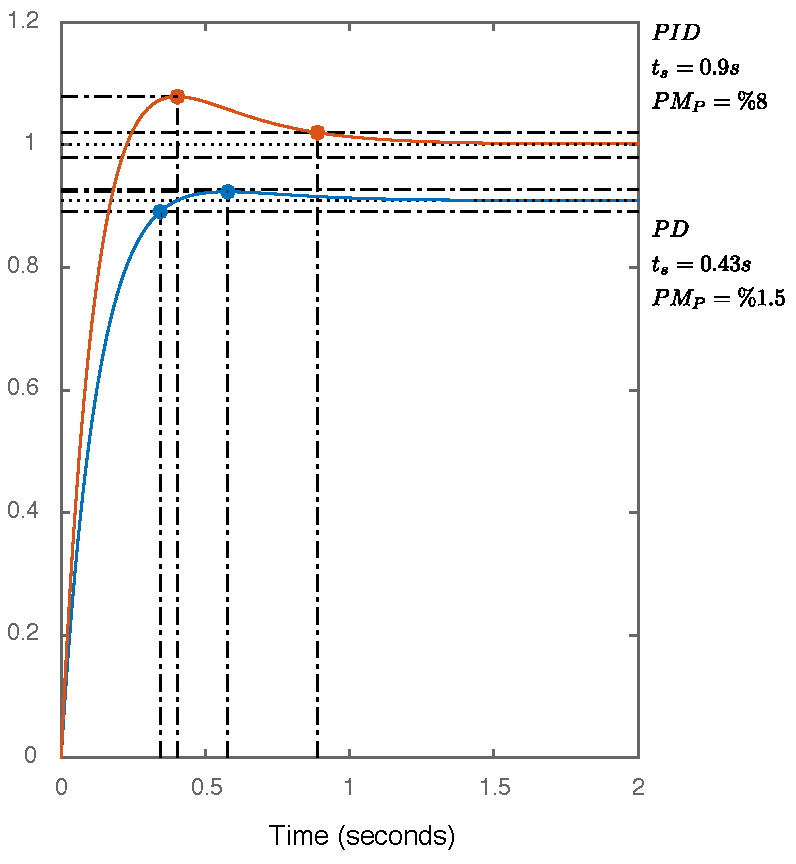
\includegraphics[width=0.4\textwidth]{PDvsPID}
    \end{center}
  \end{minipage}

\vspace{12 pt}

We can clearly see the qualitative differences between the designed PD
and PID controllers. For this specific controllers, we can see that 
PD has much better transient performance and PID is superior in
steady-state performance. Note that PID completely eliminates the
steady-state error and it is certainly possible to improve the
steady-state performance of PD controller by increasing its gain.

On the other hand in PID controller, if we locate both zeros to the
left of the pole at $-3$ location (\textbf{left as a practice}). we 
would obtain better root-locus picture (in terms of pole locations
 with better transient performance). However, the main trade-off will
be the substantially increased gain values, which is already much
larger then the designed P and PD controllers.

\vspace{12pt}

\textbf{Example:} Design a controller $C(s)$ for the following
feedback-system such that dominant closed-loop poles
has a damping ratio of $\zeta = 1/\sqrt{2}$ and damped natural
frequency of $\omega_d = 2 rad/s$.

\vspace{12 pt}

  \begin{minipage}[h]{1\linewidth}
    \begin{center}
      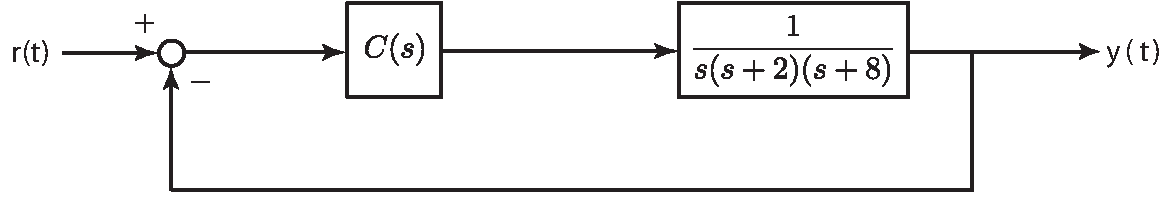
\includegraphics[width=0.6\textwidth]{example}
    \end{center}
  \end{minipage}

\vspace{12 pt}

\textbf{Solution:} Since there is no steady-state requirement 
and the goal is to locate the dominant poles to a specific location,
first natural choice of a controller is a PD controller. We know that 
PD controller can be written in the following forms
%
\begin{align*}
 C(s) = K_P + K_D s = K_D (s + \alpha)
\end{align*}
% 
and the open-loop transfer function takes the form
%
\begin{align*}
  G_{OL}(s) = K_D \frac{s + \alpha}{s (s+2) (s+8)}
\end{align*}
%
Desired pole location can be explicitly computed as
%
\begin{align*}
    \tan \phi = \frac{\sqrt{1 - \zeta^2}}{\zeta} = 1 \\
    p_{1,2} = -2 \pm 2 j 
\end{align*}
%
Now let's try to compute $\alpha$ using the angle condition
since we want the specified pole to be on the root-locus
%
\begin{align*}
  \angle [ G(s) ]_{s=p} &= (2 k + 1) \pi \ k \in \mathbb{Z}
\\
,
\\
  \angle [ G(p) ] &= \angle [ p + \alpha ] - \left( \angle [ p ] +
  \angle [ p + 2 ] + \angle [ p + 8 ] \right) 
\\
&= \angle [ (-2 + \alpha) \pm 2 j ]  - \left( \frac{3 \pi}{4} +
  \frac{\pi}{2} + \arctan (1/3) \right) 
\\
&= \angle [ (-2 + \alpha) \pm 2 j ]  + \frac{3 \pi}{4} - \arctan (1/3) 
\\
,
\\
\angle [ (-2 + \alpha) \pm 2 j ] &= \frac{\pi}{4} - \arctan (1/3)   
\\
,
\\
\Rightarrow \frac{2}{\alpha - 2} &= \arctan \left( \frac{\pi}{4} + \arctan
  (1/3) \right) = 2
\\
\\
\Rightarrow \alpha = 3
\end{align*}
%
Note that direct complex algebra could provide a simpler computational
process. Now given that $\alpha = 3$, let's draw the root locus.
We can see that the desire dominant pole locations are satisfied 
when $K_P = 48$ and $K_D = 16$. 
%
\vspace{3 pt}

  \begin{minipage}[h]{1\linewidth}
    \begin{center}
      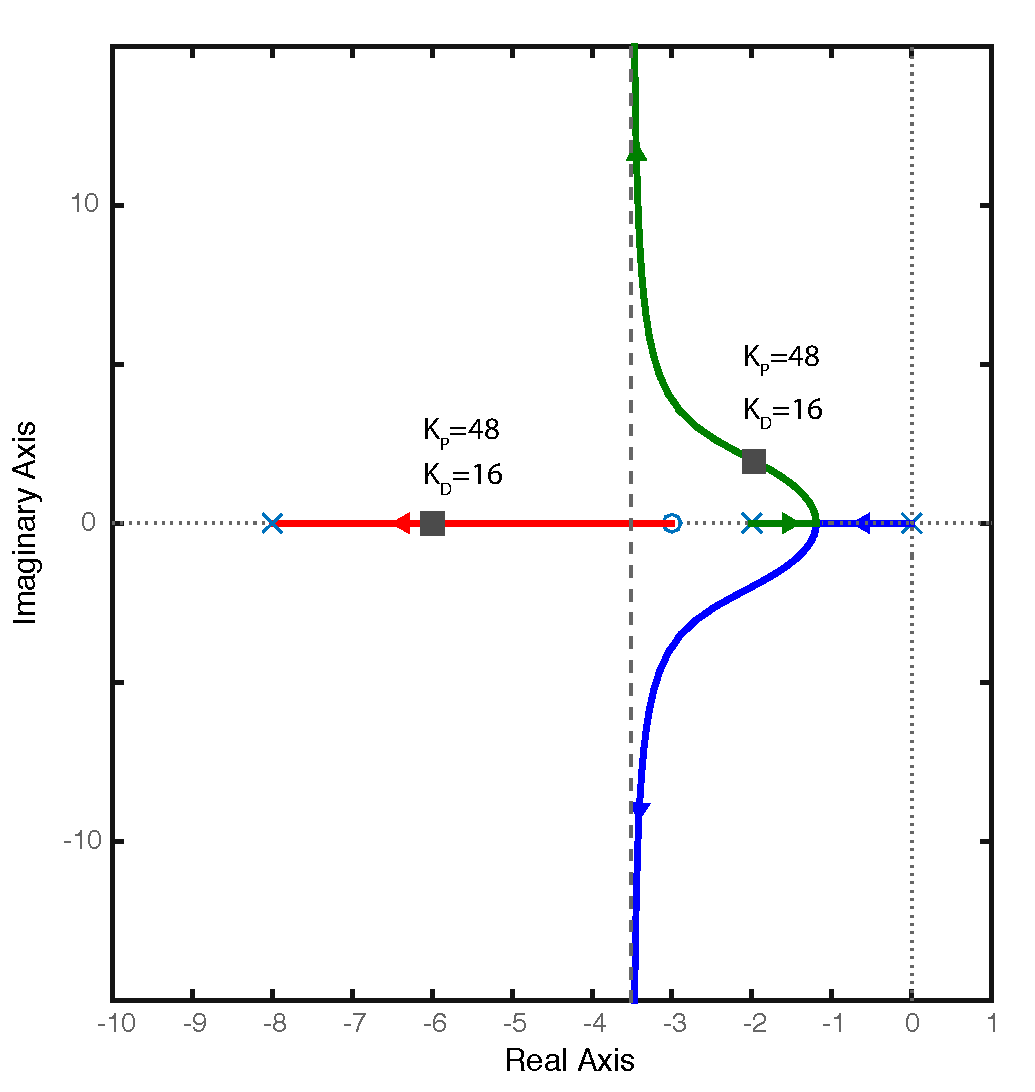
\includegraphics[width=0.4\textwidth]{PDdesignLocus}
    \end{center}
  \end{minipage}

\vspace{3 pt}

\vspace{12 pt}

\textbf{Example:} Design a controller for the following
feedback-system such that dominant closed-loop poles
has a damping ratio of $\zeta = 1/\sqrt{2}$ and damped natural
frequency of $\omega_d = 2 rad/s$, system has zero
unit step steady-state error. 

\vspace{6 pt}

  \begin{minipage}[h]{1\linewidth}
    \begin{center}
      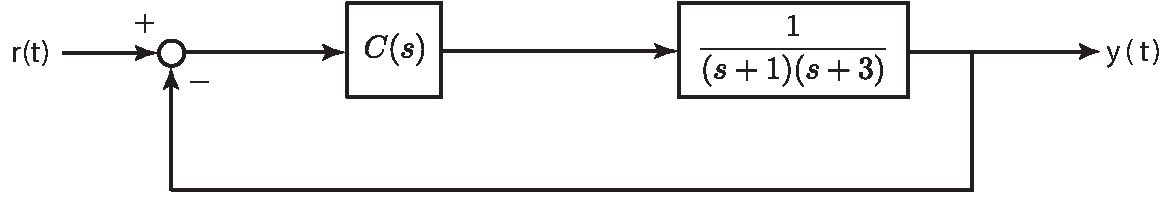
\includegraphics[width=0.55\textwidth]{example2}
    \end{center}
  \end{minipage}

\vspace{6 pt}

\textbf{Solution:} Since the requirement imposes zero steady-state
error we have to implement an I action. Let's test a PI controller 
first. 

%
\begin{align*}
 C(s) = K_P + K_I \frac{1}{s} = K_I \frac{s + \alpha}{s}
\end{align*}
% 
and the open-loop transfer function takes the form
%
\begin{align*}
  G_{OL}(s) = K_I \frac{s + \alpha}{s (s+1) (s+3)}
\end{align*}
%
Now let's try to compute $\alpha$ using the angle condition
since we want the specified pole to be on the root-locus
%
\begin{align*}
  \angle [ G(s) ]_{s=p} &= (2 k + 1) \pi \ k \in \mathbb{Z}
\\
,
\\
  \angle [ G(p) ] &= \angle [ p + \alpha ] - \left( \angle [ p ] +
  \angle [ p + 1 ] + \angle [ p +  3] \right) 
\\
&= \angle [ p + \alpha ]  - \left( \frac{3 \pi}{4} + \pi - \arctan(2)
  + \arctan(2) \right) 
\\
&= \angle [ p + \alpha ]  + \frac{\pi}{4} 
\\
,
\\
\angle [ (-2 + \alpha) \pm 2 j ] &= \frac{3 \pi}{4} \quad \Rightarrow
                                   \alpha = 0 \ (????????)
\end{align*}
% 
This implies that a PI controller can not satisfy the requirements.
Now let's try to designa PID controller. 
%
\begin{align*}
 C(s) &= K_D s + K_P + K_I \frac{1}{s} = 
= K_D  \frac{ s^2 +   (K_P/K_D) s  + (K_I/K_D)  }{s}
\\
&= K_D \frac{ (s+\alpha) (s + \beta) }{s}
\end{align*}
%
Now we have two parameters to satisfy angle condition. Let's simplify
the process and let $\alpha = \beta$, thus the PID controller has the
following form
%
\begin{align*}
 C(s) 
&= K_D \frac{(s+\alpha)^2}{s}
\end{align*}
%
Now let's try to compute $\alpha$ using the angle condition
%
\begin{align*}
  \angle [ G_{OL}(s) ]_{s=p} &= (2 k + 1) \pi \ k \in \mathbb{Z}
\\
,
\\
  \angle [ G_{OL}(p) ] &= 2 \angle [ p + \alpha ] - \left( \angle [ p ] +
  \angle [ p + 1 ] + \angle [ p +  3] \right) 
\\
&= 2 \angle [ p + \alpha ]  - \left( \frac{3 \pi}{4} + \pi - \arctan(2)
  + \arctan(2) \right) 
\\
&= 2 \angle [ p + \alpha ]  + \frac{\pi}{4} 
\\
,
\\
\angle [ (-2 + \alpha) \pm 2 j ] &= \frac{3 \pi}{8} \quad \Rightarrow
                                   \alpha = 2.8284 
\end{align*}
%
Now let's compute $K_D$ using magnitude condition
%
\begin{align*}
  K_D = \frac{1}{| G_{OL}(-2 + 2 j) |} = 3.018
\end{align*}
%
then we can compute $K_P$ and $K_I$ gains 
\begin{align*}
& K_D \left( s^2 +   (K_P/K_D) s  + (K_I/K_D)  \right)
= K_D (s+\alpha)^2 = K_D ( s^2 + 5.657 s + 8)
\\
& K_I = 24.12
\\
& K_P = 17.07
\end{align*}
%
Let's compute closed-loop transfer function and associated
closed loop-poles
%
\begin{align*}
  T(s) &= \frac{ 3.018 s^2 + 17.07 s + 24.12 }{ s^3 + 7.018 s^2 + 20.07
  s + 24.12  }
  \\
  p_{1,2} &= -2 \pm 2 j
\\
p_{3} &= -3.0144
\end{align*}
%
We can see that the poles that are closer to the origin are placed at 
desired locations, but we can also see that third pole is not
far away enough to conclude the dominance. Now let's plot the
step-response of the closed-loop system,

\vspace{6 pt}

  \begin{minipage}[h]{1\linewidth}
    \begin{center}
      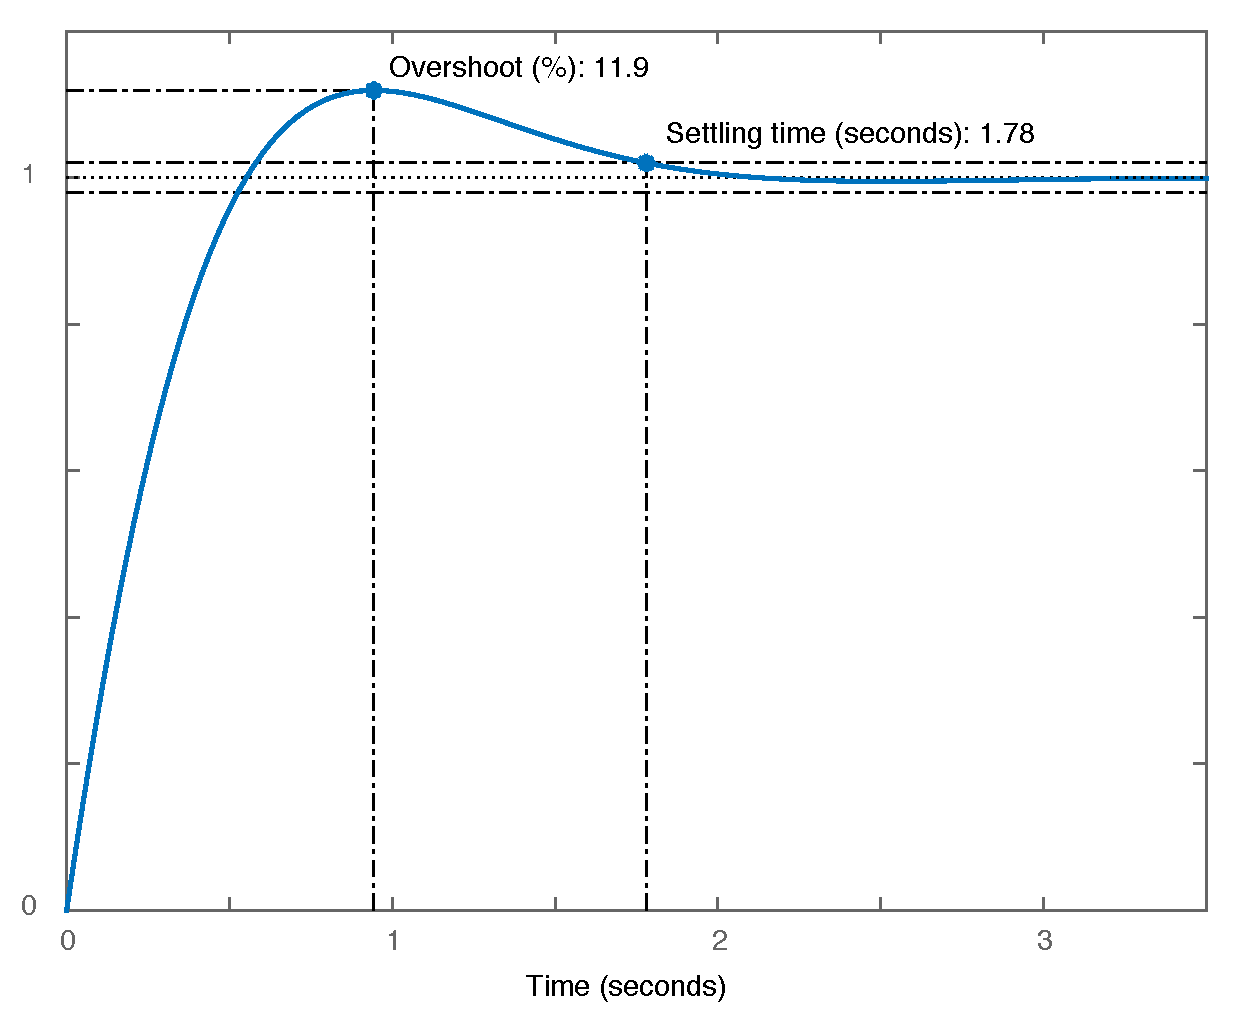
\includegraphics[width=0.4\textwidth]{PIDexample}
    \end{center}
  \end{minipage}

\vspace{6 pt}

Based on the dominant pole locations, we would expect a settling
time value of $t_{s} \approx 2 s$, while the actual settling tim is 
approximatelly $1.8 s$. On the other hand the over-shoot expectation
based on the pole location is $PM_P = \%4$, where as in the simulation
we observe $\%12$ maximum overs-hoot. Note that, we observed similar
``errors'' due to closed-loop zero dynamics even in the cases where 
system has only to complex-conjugate poles. For this reason, PID
controller fairly satisfies tha design requirements. 


% **** This ENDS THE EXAMPLES. DON'T DELETE THE FOLLOWING LINE:
\end{document}